\documentclass[border=2pt]{standalone}
\usepackage{mathptmx}\usepackage[scaled=0.92]{helvet}
\usepackage{xcolor}
\usepackage{tikz}
\usetikzlibrary{arrows.meta,positioning,fit,calc}
\usepackage{pgfplots}
\pgfplotsset{compat=1.17}
\definecolor{mapis}{RGB}{164,18,63}
\definecolor{slgray}{RGB}{138,148,156}
\begin{document}
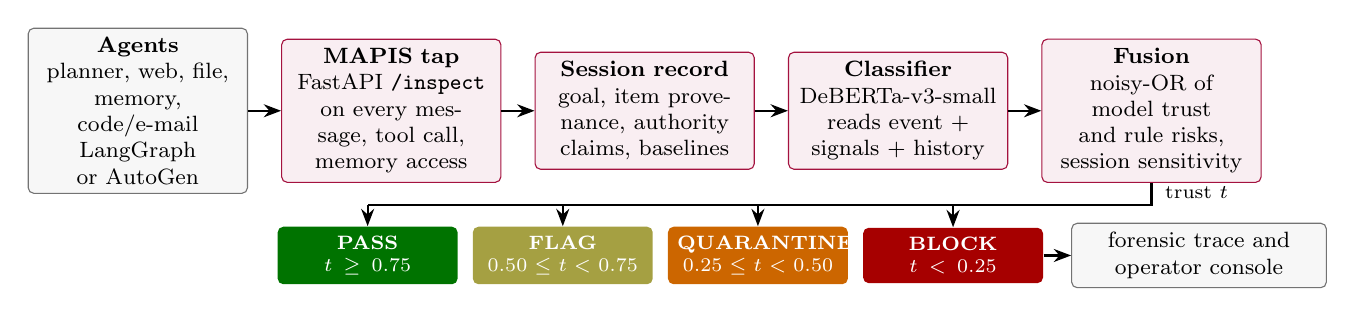
\begin{tikzpicture}[font=\footnotesize, node distance=0.42cm,
 box/.style={draw=black!55, rounded corners=2pt, align=center, minimum height=1.25cm, text width=2.55cm, fill=black!3},
 hot/.style={box, draw=mapis, fill=mapis!7},
 tier/.style={rounded corners=2pt, align=center, minimum height=0.62cm, text width=2.05cm, text=white, font=\scriptsize\bfseries},
 ar/.style={-{Stealth[length=2.2mm]}, thick}]
\node[box] (ag) {\textbf{Agents}\\planner, web, file,\\memory, code/e-mail\\LangGraph or AutoGen};
\node[hot, right=of ag] (tap) {\textbf{MAPIS tap}\\FastAPI \texttt{/inspect} on every message, tool call, memory access};
\node[hot, right=of tap] (rec) {\textbf{Session record}\\goal, item provenance, authority claims, baselines};
\node[hot, right=of rec] (clf) {\textbf{Classifier}\\DeBERTa-v3-small reads event + signals + history};
\node[hot, right=of clf] (fuse) {\textbf{Fusion}\\noisy-OR of model trust and rule risks, session sensitivity};
\foreach \a/\b in {ag/tap,tap/rec,rec/clf,clf/fuse} \draw[ar] (\a) -- (\b);
\node[tier, fill=green!45!black, below=0.55cm of tap, xshift=-0.3cm] (p) {PASS\\$t\ge0.75$};
\node[tier, fill=yellow!60!black, right=0.18cm of p] (f) {FLAG\\$0.50\le t<0.75$};
\node[tier, fill=orange!80!black, right=0.18cm of f] (q) {QUARANTINE\\$0.25\le t<0.50$};
\node[tier, fill=red!65!black, right=0.18cm of q] (b) {BLOCK\\$t<0.25$};
\node[box, text width=3.0cm, minimum height=0.62cm, right=0.35cm of b] (tr) {forensic trace and operator console};
\coordinate (bus) at ($(fuse.south)+(0,-0.28)$);
\draw[thick] (fuse.south) -- (bus) -- (bus -| p.north);
\node[font=\scriptsize, anchor=west] at ($(fuse.south)+(0.05,-0.12)$) {trust $t$};
\foreach \x in {p,f,q,b} \draw[ar] (bus -| \x.north) -- (\x.north);
\draw[ar] (b) -- (tr);
\end{tikzpicture}
\end{document}
